\chapter{Lực, quark và các đa tuyến hadron đầu tiên}

\section{Hạt, trường và cạnh thứ ba còn thiếu}

Sóng là các cấu hình của trường, nên trong thảo luận hiện tại hai cách mô tả này liên hệ chặt chẽ với nhau. Cơ học lượng tử nói rằng năng lượng trong một sóng như vậy xuất hiện dưới dạng những đơn vị rời rạc, không thể chia nhỏ. Những đơn vị ấy là các lượng tử của nó, và các lượng tử của một trường chính là điều ta gọi là các hạt của trường đó. Với mối liên hệ ấy trong tay, ta đã bàn đến các phương trình sóng, các nguyên lý tác dụng, và những tính chất khái quát do hạt mang: năng lượng, động lượng, spin, và sự phân biệt boson--fermion. Fermion chống lại việc cùng chiếm một trạng thái; boson có thể tụ lại và ngưng tụ vào một trạng thái.

Một Lagrangian lượng tử cũng ghi lại các tương tác. Tích của các trường biểu diễn những đỉnh mà tại đó các hạt đi vào và đi ra. Chẳng hạn, một hạng chứa bốn lũy thừa của một trường biểu diễn một đỉnh tương tác bốn chân. Đó là cách nguyên lý tác dụng trở thành một bản liệt kê cô đọng các quá trình hạt có thể xảy ra.

Nhiệm vụ tiếp theo là gọi tên các hạt---không hẳn từng hạt một, mà theo từng họ---và gán cho mỗi họ một chút diện mạo riêng: các tính chất, các tương tác và vị trí của nó trong vật lý thông thường. Tuy nhiên, trước khi lập danh sách đó, một cạnh của tam giác khái niệm vẫn còn thiếu:
\begin{itemize}
\item các hạt,
\item các trường mà những hạt ấy là lượng tử của chúng,
\item các lực gắn với những quá trình trao đổi có sự tham gia của chính các lượng tử ấy.
\end{itemize}

Từ \emph{cơ bản} phải vẫn chỉ mang tính tạm thời. Mọi định nghĩa có vẻ hợp lý về một hạt là cơ bản chứ không phải hợp thành rốt cuộc đều gặp một trường hợp khó nắm bắt, và ta sẽ quay lại vấn đề đó. Còn bây giờ, hãy giả sử các trường cơ bản tồn tại và gọi các lượng tử của chúng là các hạt cơ bản. Nếu điện trường sinh ra lực điện và trường hấp dẫn sinh ra lực hấp dẫn, thì trường electron cũng phải tham gia vào các lực. Tam giác chỉ có thể khép kín nếu lực có một mô tả bằng hạt cũng như một mô tả bằng trường.

Vì thế ta sẽ suy ra logic của lực hai lần. Trước hết ta dùng năng lượng trường cổ điển; sau đó ta hỏi cùng tương tác ấy xuất hiện ra sao khi một trường được phân giải thành các lượng tử. Chỉ sau khi chiếc cầu nối ấy đã vững chắc thì bản liệt kê các hạt mới bắt đầu.

\section{Lực từ năng lượng trường trong điện động lực học cổ điển}

Đặt hai điện tích trong không gian. Một cách để tìm lực giữa chúng là viện dẫn định luật nghịch đảo bình phương. Một cách bộc lộ bản chất hơn là hỏi các điện tích làm gì với không gian: chúng tạo ra các điện trường, và các trường ấy tích trữ năng lượng.

Thật hữu ích khi tách mỗi điện tích khỏi dạng không gian của trường do nó tạo ra,
\begin{equation}
\mathbf E_i=q_i\widehat{\mathbf E}_i,
\end{equation}
mặc dù không điều gì phụ thuộc vào việc có giữ ký hiệu mũ hay không. Khi có mặt cả hai điện tích, tính tuyến tính cho
\begin{equation}
\mathbf{E}=\mathbf{E}_1+\mathbf{E}_2.
\end{equation}
Bỏ qua lựa chọn đơn vị, năng lượng của trường tĩnh điện có dạng
\begin{equation}
U_{\text{field}}\propto\int d^3x\,\mathbf{E}^2.
\end{equation}
Thế tổng của hai trường vào, ta được
\begin{align}
U_{\text{field}}
&\propto\int d^3x\,(\mathbf{E}_1+\mathbf{E}_2)^2 \\
&\propto\int d^3x\,\bigl(\mathbf{E}_1^2+\mathbf{E}_2^2
  +2\mathbf{E}_1\!\cdot\!\mathbf{E}_2\bigr).
\end{align}

Hai hạng đầu là tự năng. Tịnh tiến một trong hai điện tích sẽ mang trường của nó đi theo và không làm thay đổi tích phân tương ứng. Năng lượng ấy đóng góp, thông qua \(E=mc^2\), vào khối lượng đo được của hạt mang điện cô lập. Việc tự năng đó được hấp thụ vào khối lượng đo được như thế nào thuộc về chủ đề tái chuẩn hóa sẽ bàn sau. Không phần năng lượng nào độc lập với vị trí như vậy góp vào lực giữa hai hạt.

Hạng chéo thì khác. Nó không thuộc riêng hạt nào và chỉ tồn tại khi cả hai trường đều hiện diện. Nếu đưa các điện tích ra rất xa nhau, những vùng trường đáng kể của chúng hầu như không chồng lấp. Khi các điện tích tiến lại gần, độ chồng lấp thay đổi. Vì thế năng lượng tương tác phụ thuộc cấu hình tỉ lệ với
\begin{equation}
U_{\text{int}}(r)\propto q_1q_2\int d^3x\,
\widehat{\mathbf E}_1\!\cdot\!\widehat{\mathbf E}_2.
\end{equation}
Với hai điện tích điểm cách nhau \(r\), tính tích phân cho ta sự phụ thuộc quen thuộc
\begin{equation}
U_{\text{int}}(r)\propto\frac{q_1q_2}{r}.
\end{equation}
Lực hướng tâm là gradient âm của nó,
\begin{equation}
\mathbf F_{12}=-\boldsymbol\nabla_{\mathbf r}U_{\text{int}},
\qquad
|\mathbf F_{12}|\propto\frac{|q_1q_2|}{r^2}.
\end{equation}
\editorialnote{Lập luận bằng lời đồng nhất hạng chéo với lực Coulomb nghịch đảo bình phương mà không dừng lại ở thế năng. Bước trung gian chuẩn \(U_{\mathrm{int}}\propto1/r\) được viết tường minh ở đây để gradient của nó cho ra lực \(1/r^2\) đã nêu.}

Định luật lực đã trở thành đạo hàm của phần năng lượng trường phụ thuộc vào vị trí tương đối. Khi ở xa nhau, hai vật về thực chất là độc lập. Đưa chúng lại gần nhau thì trường giữa chúng được sắp xếp lại; độ biến thiên năng lượng do đó chính là tương tác.

Nhưng nếu một trường có thể được phân giải thành các lượng tử, thì đó chưa thể là hết câu chuyện. Cùng lực ấy phải có một mô tả bằng ngôn ngữ hạt.

\section{Trao đổi phân tử: hai proton và một electron}

Trước khi quay lại điện động lực học, hãy xét một hệ trong đó sự trao đổi dễ hình dung hơn: hai proton và một electron. Trao đổi chỉ là một trong vài nguồn gốc của lực phân tử, nhưng ví dụ này làm lộ rõ mối liên hệ giữa trao đổi, năng lượng và lực. Nó không được đưa ra như một sự thay thế cho điện động lực học lượng tử.

Nếu có một proton hiện diện còn proton kia ở xa vô hạn, electron có thể chiếm trạng thái cơ bản kiểu hydro lấy tâm tại proton thứ nhất. Hàm sóng của nó khu trú gần tâm lực đó.

\begin{figure}[h]
\centering
\includegraphics[width=0.72\textwidth]{lecture_01_figure_02.png}

\medskip

\begin{tikzpicture}[scale=0.95]
\draw (-0.2,0) -- (6.4,0);
\fill (1.3,0) circle (2pt);
\draw[smooth] plot coordinates {(0.1,0.15) (0.8,1.15) (1.5,1.75) (2.2,1.1) (3.0,0.35) (3.8,0.12)};
\node at (1.3,-0.35) {$p$};
\node at (2.7,1.55) {$\psi_1(x)$};
\end{tikzpicture}
\caption{Hàm sóng trạng thái cơ bản kiểu hydro khu trú gần một proton.}
\lectureframe{00:14:32}
\end{figure}
\editorialnote{Nhãn \(\psi_1(x)\) trong hình vẽ lại dùng để chỉ biên dạng khu trú được mô tả tại 00:14:30--00:14:32; nó không được sao chép từ một nhãn trên bảng còn đọc được.}

Bây giờ đặt proton thứ hai ở một khoảng cách lớn nhưng hữu hạn. Do đối xứng, có một trạng thái khu trú thứ hai với cùng năng lượng một tâm, lần này lấy tâm tại proton bên phải.

\begin{figure}[h]
\centering
\includegraphics[width=0.78\textwidth]{lecture_01_figure_03.png}

\medskip

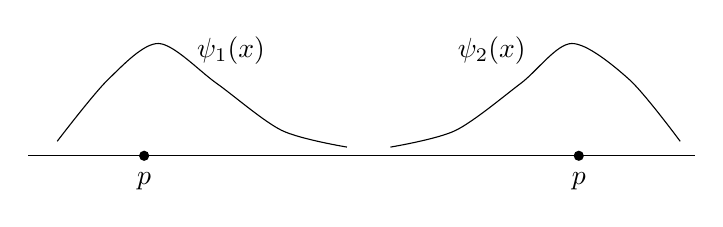
\begin{tikzpicture}[scale=0.92]
\draw (-0.2,0) -- (9.0,0);
\fill (1.4,0) circle (2pt);
\fill (7.4,0) circle (2pt);
\draw[smooth] plot coordinates {(0.2,0.2) (0.9,1.05) (1.6,1.55) (2.4,1.0) (3.3,0.35) (4.2,0.12)};
\draw[smooth] plot coordinates {(4.8,0.12) (5.7,0.35) (6.6,1.0) (7.3,1.55) (8.1,1.05) (8.8,0.2)};
\node at (1.4,-0.35) {$p$};
\node at (7.4,-0.35) {$p$};
\node at (2.6,1.45) {$\psi_1(x)$};
\node at (6.2,1.45) {$\psi_2(x)$};
\end{tikzpicture}
\caption{Hai biên dạng khu trú được dùng để tạo thành chồng chập cân bằng sau khi cho phép xuyên hầm.}
\lectureframe{00:17:54}
\end{figure}
\editorialnote{Các nhãn \(\psi_1(x)\) và \(\psi_2(x)\) xác định hai biên dạng được bàn đến tại 00:17:41--00:17:56; các ký hiệu là những nhãn sơ đồ được thêm vào cho dễ đọc.}

Ở khoảng cách vô hạn, hai trạng thái là suy biến: khu trú electron ở bên trái hay bên phải đều tốn cùng một năng lượng. Ở khoảng cách hữu hạn, một quá trình mới trở nên khả dĩ. Electron có thể xuyên hầm qua vùng bị cấm cổ điển từ tâm này sang tâm kia. Nếu cố quan sát một quỹ đạo xuyên qua hàng rào, ta sẽ làm nhiễu trạng thái; ``nhảy'' là một mô tả của diễn hóa lượng tử, không phải một thước phim về một quỹ đạo cổ điển.

Ở trạng thái cân bằng, xác suất tìm thấy electron gần mỗi proton là như nhau. Vì vậy việc chuẩn hóa đưa vào hệ số \(1/\sqrt2\), và trạng thái cân bằng năng lượng thấp hơn xấp xỉ là
\begin{equation}
\psi_+(x)\approx \frac{\psi_1(x)+\psi_2(x)}{\sqrt2}.
\end{equation}

Dấu xấp xỉ là quan trọng. Hàm sóng hai tâm thực sự không chính xác là tổng của hai obitan kiểu hydro không bị nhiễu; nó tự điều chỉnh trong vùng chồng lấp. Điều cần dùng ở đây là trạng thái cân bằng đối xứng nằm thấp hơn năng lượng một tâm cô lập. Theo ngôn ngữ Hamiltonian, các cấu hình trái và phải được ghép với nhau bởi một phần tử ma trận ngoài đường chéo. Việc cho phép electron chiếm chồng chập kết hợp của chúng đã làm hạ năng lượng.

\section{Từ năng lượng hạ thấp đến một lực hiệu dụng}

Ở khoảng cách proton lớn, phần đóng góp do electron gây ra \(E_e(r)\) tiến tới giá trị của nguyên tử tách rời. Ở khoảng cách nhỏ hơn, xuyên hầm và chồng chập làm hạ đóng góp ấy. Thế năng đầy đủ của hệ hai proton--một electron còn phải chứa cả lực đẩy trực tiếp giữa các proton,
\begin{equation}
V_{\mathrm{tot}}(r)=V_{pp}(r)+E_e(r).
\end{equation}

Điều này nối lại ví dụ phân tử với lập luận về năng lượng trường. Những phác họa hàm sóng và đường cong định tính của \(E_e(r)\) là hai cách nhìn của cùng một phép tính; trạng thái cân bằng được quyết định bởi tổng \(V_{\mathrm{tot}}(r)\).

\begin{figure}[h]
\centering
\includegraphics[width=0.78\textwidth]{lecture_01_figure_04.png}

\medskip

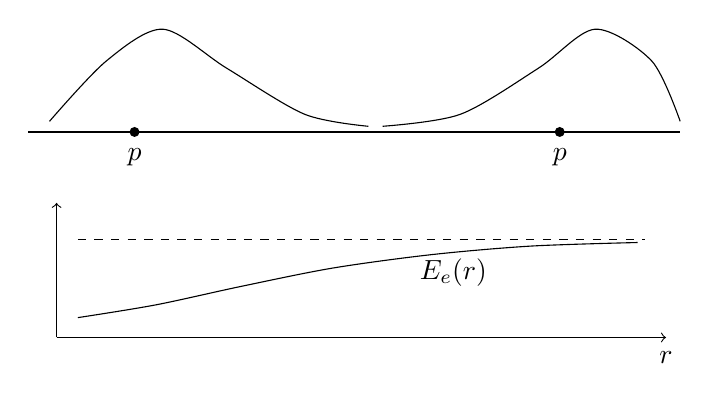
\begin{tikzpicture}[scale=0.9]
\draw (-0.2,3.0) -- (9.0,3.0);
\fill (1.3,3.0) circle (2pt);
\fill (7.3,3.0) circle (2pt);
\draw[smooth] plot coordinates {(0.1,3.15) (0.9,4.0) (1.7,4.45) (2.6,3.9) (3.7,3.25) (4.6,3.08)};
\draw[smooth] plot coordinates {(4.8,3.08) (5.9,3.25) (7.0,3.9) (7.8,4.45) (8.6,4.0) (9.0,3.15)};
\node at (1.3,2.65) {$p$};
\node at (7.3,2.65) {$p$};

\draw[->] (0.2,0.1) -- (0.2,2.0);
\draw[->] (0.2,0.1) -- (8.8,0.1);
\draw[dashed] (0.5,1.48) -- (8.5,1.48);
\draw[smooth] plot coordinates {(0.5,0.38) (1.6,0.56) (2.8,0.82) (4.1,1.08) (5.5,1.27) (6.9,1.39) (8.4,1.44)};
\node at (5.8,1.02) {$E_e(r)$};
\node at (8.8,-0.18) {$r$};
\end{tikzpicture}
\caption{Ở trên là sự chồng lấp của các hàm sóng và ở dưới là năng lượng do electron gây ra. Đường cong này tăng dần về tiệm cận của nguyên tử tách rời khi \(r\) tăng; thế năng tổng của các proton còn phải bao gồm lực đẩy Coulomb của chúng.}
\lectureframe{00:20:28}
\end{figure}
\editorialnote{Các nhãn \(E_e(r)\) và \(r\) xác định đường cong năng lượng và khoảng cách được bàn đến tại 00:19:12--00:20:38; khung hình còn lại trên bảng không cho đọc được các nhãn trục đó.}

Hai lực tương ứng suy ra từ các gradient năng lượng,
\begin{equation}
F_{e}(r)=-\frac{dE_e}{dr},
\qquad
F_{\mathrm{tot}}(r)=-\frac{dV_{\mathrm{tot}}}{dr}.
\end{equation}
Vì vậy hệ được đẩy về phía năng lượng toàn phần thấp hơn. Ở những khoảng mà \(E_e(r)\) giảm khi các proton tiến lại gần nhau, trao đổi cung cấp một đóng góp hút; việc có tồn tại một khoảng cách liên kết hay không phụ thuộc vào sự cạnh tranh của nó với \(V_{pp}(r)\). Đây là cơ chế cơ bản đứng sau liên kết cộng hóa trị: electron được chia sẻ vì trạng thái chia sẻ là thuận lợi về năng lượng.

Trong phép tính cổ điển, sự chồng lấp của các điện trường làm thay đổi năng lượng. Ở đây, hai tâm lực cho phép một trạng thái lượng tử thấp hơn. Cả hai cơ chế đều sinh ra lực vì năng lượng cân bằng phụ thuộc vào cấu hình.

Ngôn ngữ trao đổi có thể được tóm tắt bằng một hình phác đường thế giới. Không được đọc nó như một quỹ đạo đã quan sát; nó biểu diễn các biên độ để electron gắn với proton này hay proton kia.

\begin{figure}[h]
\centering
\begin{tikzpicture}[scale=1.0]
\draw (0,0) -- (0,4.4);
\draw (4.8,0) -- (4.8,4.4);
\draw (0,0.9) .. controls (1.6,1.7) and (3.2,1.7) .. (4.8,2.5);
\draw (4.8,2.9) .. controls (3.2,2.1) and (1.6,2.1) .. (0,3.9);
\node at (0,-0.35) {$p$};
\node at (4.8,-0.35) {$p$};
\node at (2.35,1.55) {$e^-$};
\node at (2.35,2.55) {$e^-$};
\end{tikzpicture}
\caption{Trao đổi electron giữa hai đường thế giới proton, được hiểu như một sơ đồ các biên độ lượng tử chứ không phải một đường đi bị theo dõi.}
\end{figure}

\begin{classroomqa}
\audiencequestion{Có thể hiểu lực hút một cách đơn giản chỉ như electron che chắn hoặc làm giảm điện tích proton không?\lecturetimestamp{00:23:26}}
\lecturerresponse{Không. Hình dung theo kiểu giảm điện tích không phải là bức tranh đúng cho hiệu ứng này. Sự kiện cốt yếu là việc cộng hai hàm sóng khu trú tạo ra một trạng thái có năng lượng thấp hơn đôi chút so với từng trạng thái khu trú riêng rẽ.}
\end{classroomqa}

\begin{classroomqa}
\audiencequestion{Đây có phải là điều Feynman muốn nói khi bảo rằng ``ánh sáng thích ánh sáng'' không?\lecturetimestamp{00:23:51}}
\lecturerresponse{Không. Câu đó nhiều khả năng nói về thống kê Bose: photon ưu tiên các trạng thái chung, còn electron tuân theo nguyên lý loại trừ. Hiệu ứng phân tử ở đây là sự xuyên hầm giữa hai tâm.}
\end{classroomqa}

Hai proton vẫn đẩy nhau về mặt tĩnh điện. Trao đổi có tầm ngắn hơn tương tác Coulomb, nên phải xét thế năng tổng chứ không phải từng phần đóng góp riêng lẻ. Tuy vậy, ở những khoảng cách thích hợp, ion phân tử \(\mathrm H_2^+\) vẫn là hệ liên kết; trong một hệ trung hòa hai electron, lực đẩy điện tích tầm xa không còn và liên kết cộng hóa trị lại càng quen thuộc hơn.

\begin{classroomqa}
\audiencequestion{Việc đặt electron giữa hai proton có chủ yếu làm giảm lực đẩy tĩnh điện của chúng không?\lecturetimestamp{00:24:33}}
\lecturerresponse{Nó có làm giảm lực đẩy đi một ít, nhưng đó không phải hiệu ứng chính. Trao đổi electron là một lực tầm ngắn hơn lực đẩy Coulomb. Nó thấy rõ nhất trong một hệ trung hòa hai electron, nơi lực điện tĩnh tầm xa giữa các nguyên tử không còn nhưng xuyên hầm vẫn tạo ra lực hút.}
\end{classroomqa}

\begin{classroomqa}
\audiencequestion{Ion phân tử mang điện dương \(\mathrm H_2^+\), chỉ với một electron, có thực sự là một hệ liên kết không?\lecturetimestamp{00:26:06}}
\lecturerresponse{Có. Ở khoảng cách đủ nhỏ, lực hút do trao đổi đủ mạnh để thắng lực đẩy Coulomb proton--proton.}
\end{classroomqa}

\begin{classroomqa}
\audiencequestion{Cách sắp xếp hai tâm có tạo ra một lực thứ ba không?\lecturetimestamp{00:26:24}}
\lecturerresponse{Không có lực cơ bản mới nào được đưa vào. Phương trình Schr\"odinger trong thế kết hợp của hai proton có một năng lượng cân bằng khác với bài toán một tâm; đạo hàm của năng lượng đã thay đổi ấy chính là lực hiệu dụng.}
\end{classroomqa}

\begin{classroomqa}
\audiencequestion{Sự hạ năng lượng này có phải là một ví dụ của vướng víu lượng tử không?\lecturetimestamp{00:27:06}}
\lecturerresponse{Không theo nghĩa thông thường của hai hạt: chỉ cần một electron là đủ. Đặc trưng toán học liên quan là một phần tử ma trận Hamiltonian ngoài đường chéo ghép các trạng thái trái và phải.}
\end{classroomqa}

\begin{classroomqa}
\audiencequestion{Điều gì xảy ra với sự trao đổi ở nhiệt độ cao?\lecturetimestamp{00:27:37}}
\lecturerresponse{Ở nhiệt độ cực cao, electron bị ion hóa và không còn liên hệ gì với phân tử nữa. Ở năng lượng kích thích thấp hơn, nó có thể chiếm một obitan lớn hơn, làm thay đổi độ chồng lấp và do đó làm thay đổi lực. Đây là một hiệu chỉnh phụ thuộc trạng thái, không phải một cơ chế tổng quát mới.}
\end{classroomqa}

\section{Sự trao đổi photon và các mục đầu tiên của bảng}

Có thể mô tả lực Coulomb bằng cùng ngôn ngữ trao đổi đó không? Một hạt mang điện tương tác với trường điện từ, mà các lượng tử của trường này là photon. Trong mô tả cổ điển, ta giải tìm điện trường xung quanh điện tích. Trong lý thuyết trường lượng tử, ta phân giải tương tác đó thành sự phát xạ và hấp thụ photon.

Một hạt mang điện vật lý không chỉ đơn thuần là một điện tích trần. Trạng thái của nó là một chồng chập lượng tử chứa thành phần electron trần, một electron kèm một photon, một electron kèm hai photon, v.v. Trong ký hiệu sơ đồ hóa có chủ ý,
\begin{equation}
\begin{aligned}
\ket{e_{\mathrm{phys}}}
={}&a_0\ket e
+a_1\ket{e+\text{one photon}}
\\
&+a_2\ket{e+\text{two photons}}+\cdots .
\end{aligned}
\end{equation}
Ký hiệu này chỉ ghi lại thứ bậc các thành phần theo số photon; nó không xác định xung lượng photon cũng không cố xây dựng đầy đủ một trạng thái mang điện tương tác.
Các photon bao quanh được phát ra rồi tái hấp thụ, thay vì thoát đi như bức xạ tự do. Hiệu ứng của chúng có thể đo được, dù chúng không được phát hiện theo cùng cách như các photon lan truyền tự do. Đặt một điện tích thứ hai ở gần đó, và một photon phát ra tại điện tích này có thể được hấp thụ ở điện tích kia. Khi đó hai trạng thái mang điện đã được các photon bao quanh ấy không còn có năng lượng bằng tổng đơn giản của hai năng lượng cô lập nữa.

Phép ví trong lớp học là hai người tung hứng, mỗi người với một bộ bóng. Khi họ ở xa nhau, mỗi người tung hứng độc lập. Đưa họ lại đủ gần thì một người có thể bắt quả bóng do người kia ném. Trong ngôn ngữ giản đồ Feynman, vật được chia sẻ ấy là photon trao đổi. Phép ví này không phải là một quỹ đạo vi mô, nhưng nó nắm được vì sao sự gần nhau cho phép một quá trình mới.

Giờ ta có hai mô tả vượt quá việc chỉ học thuộc định luật Coulomb. Lý thuyết trường cổ điển cộng các trường rồi bình phương kết quả. Lý thuyết trường lượng tử cộng các biên độ trong đó các lượng tử được trao đổi. Theo nghĩa này, hạt, trường và lực tạo thành một tương ứng một-một-một. Electron trung gian cho trao đổi phân tử, photon trung gian cho trao đổi điện từ, và bất kỳ hạt nào có thể được trao đổi đều có thể đóng góp vào một lực trong một bối cảnh thích hợp. Vì vậy, phát biểu quen thuộc rằng tự nhiên có bốn tương tác cơ bản là một cách phân loại ở mức rộng hơn; còn trong ngôn ngữ trao đổi, mỗi loại hạt có thể trao đổi đều có thể tạo ra đóng góp lực hiệu dụng riêng của nó.

Cuối cùng cũng đến lúc gọi tên các hạt, liệt kê các tính chất của chúng, và nói chúng có thể tham gia những quá trình nào. Viết toàn bộ Mô hình Chuẩn ngay một lúc sẽ chỉ tạo thành một bài kiểm tra ghi nhớ dài, nên ta sẽ chia các hạt thành những nhóm nhỏ mà các thành viên có liên hệ đơn giản với nhau và học xem mỗi nhóm có thể làm gì.

Bản danh mục đầy đủ khá cồng kềnh vì ta không hiểu vì sao chính xác những hạt này tồn tại còn những hạt khả dĩ khác thì không. Tính nhất quán toán học cung cấp một số quan hệ: một khi vài thành viên của một khuôn mẫu đã tồn tại, có thể phải có thêm một thành viên khác để hoàn tất nó. Các quan hệ đó làm giảm số lượng sự kiện độc lập, nhưng chỉ với một hệ số khá khiêm tốn. Nhiều loại hạt và nhiều tham số vẫn chưa được giải thích. Hiểu cấu trúc còn dang dở ấy là điều cần thiết để hiểu những thí nghiệm về sau đang cố khám phá điều gì.

\begin{figure}[h]
\centering
\includegraphics[width=0.7\textwidth]{lecture_01_figure_05.png}
\caption{Mục đầu tiên trong bảng hạt nhận diện photon bằng \(\gamma\) và trường của nó bằng thế vectơ \(A\).}
\lectureframe{00:39:11}
\end{figure}

Sự nhận diện đầu tiên giữa trường--lượng tử là
\begin{equation}
\gamma \leftrightarrow A.
\end{equation}
Ở đây \(A\) là thế vectơ điện từ. Photon là một boson spin 1 với điện tích bằng không, số baryon bằng không và khối lượng nghỉ bằng không. Trường electron theo quy ước được ký hiệu là \(\psi_e\); các phần tạo và hủy của nó tác dụng lên các trạng thái electron và positron.

Bảng của ta ghi tên, ký hiệu hạt, trường, loại boson hay fermion, điện tích \(Q\), số baryon \(B\), và khối lượng:

\begin{table}[h]
\centering
\resizebox{\linewidth}{!}{%
\begin{tabular}{lllllll}
Tên & Ký hiệu & Trường & Loại & \(Q\) & \(B\) & Khối lượng \\
Photon & \(\gamma\) & \(A\) & boson & \(0\) & \(0\) & \(0\) \\
Electron & \(e^-\) & \(\psi_e\) & fermion & \(-1\) & \(0\) & \(0.51\,\mathrm{MeV}\) \\
Positron & \(e^+\) & \(\psi_e\) & fermion & \(+1\) & \(0\) & \(0.51\,\mathrm{MeV}\)
\end{tabular}
}%
\caption{Các mục photon và electron--positron mở đầu danh mục hạt.}
\end{table}

Mối liên hệ giữa electron và positron là hai chiều: mỗi hạt là phản hạt của hạt kia. Gọi trạng thái mang điện âm là ``hạt'' chỉ là quy ước. Ta đo điện tích theo đơn vị độ lớn của điện tích electron, nên
\begin{equation}
Q(e^-)=-1,\qquad Q(e^+)=+1.
\end{equation}
Khối lượng được đo bằng đơn vị năng lượng khi dùng \(E=mc^2\). Một electron-volt là năng lượng mà điện tích \(e\) thu được khi đi qua một hiệu điện thế một volt,
\begin{equation}
1\,\mathrm{eV}=e\,(1\,\mathrm V).
\end{equation}
Đơn vị này xuất hiện tự nhiên từ vật lý nguyên tử: như một thang nguyên tử thô, việc ion hóa hydro tốn khoảng \(13.5\,\mathrm{eV}\). Khối lượng hạt đòi hỏi hàng triệu hoặc hàng tỷ electron-volt. Khối lượng electron là
\begin{equation}
m_e c^2 \approx 0.511\,\mathrm{MeV}.
\end{equation}

\begin{classroomqa}
\audiencequestion{Khối lượng electron có phải chính xác bằng một nửa MeV không?\lecturetimestamp{00:44:02}}
\lecturerresponse{Không. Giá trị làm tròn tiện dụng \(0.51\,\mathrm{MeV}\) không bị nguyên lý nào cố định thành đúng một nửa; đó là một tham số đo được.}
\end{classroomqa}

Quá trình QED sơ cấp có một đường fermion mang điện đi vào, một đường đi ra, và một đường photon gắn vào. Sắp xếp lại hoặc đổi chéo các chân cho phép cùng một đỉnh mô tả sự phát xạ photon, sự hấp thụ photon, hoặc một quá trình có positron. Trong ký hiệu sơ đồ không hiệp biến được dùng ở đây, tương tác chứa
\begin{equation}
\mathcal{L}_{\mathrm{int}}\sim e\,\psi_e^\dagger \psi_e A.
\end{equation}
Khai triển các trường thành các toán tử tạo và hủy sinh ra những hạng hủy một electron tới, tạo một electron ra, và tạo hoặc hủy một photon. Hằng số liên kết \(e\) cung cấp một thừa số tại đỉnh. Do đó, đối với sự phát xạ photon khi một electron bị tán xạ hoặc gia tốc,
\begin{equation}
\mathcal{A}_{\mathrm{vertex}}\propto e,
\qquad
P_{\mathrm{emission}}\propto e^2.
\end{equation}
Một electron đập vào bia trong một ống tia X là một bối cảnh thực tế mà xác suất phát photon này có ý nghĩa. Những tổ hợp lặp đi lặp lại của cùng đỉnh ấy sinh ra các quá trình của điện động lực học lượng tử, kể cả độ dịch năng lượng được diễn giải là lực giữa các điện tích.

Vì vậy, một đỉnh sơ đồ là hữu ích.

\begin{figure}[h]
\centering
\begin{tikzpicture}[scale=1.0]
\fill (0,0) circle (1.5pt);
\draw (-1.6,-1.2) -- (0,0) -- (1.6,-1.2);
\draw (0,0) -- (0,1.8);
\node at (-1.8,-1.4) {$e^-$};
\node at (1.8,-1.4) {$e^-$};
\node at (0.35,1.95) {$\gamma$};
\end{tikzpicture}
\caption{Sơ đồ tôpô của đỉnh QED sơ cấp: một đường fermion mang điện đi vào, một đường đi ra, và một photon được gắn vào. Chân photon vẽ thẳng ở đây chỉ là một quy ước hình vẽ đơn giản hóa.}
\end{figure}

Đóng góp trao đổi vào lực nối hai đỉnh như vậy:

\begin{figure}[h]
\centering
\begin{tikzpicture}[scale=1.0]
\draw (0,0) -- (0,4.0);
\draw (4.8,0) -- (4.8,4.0);
\draw (0,2.0) -- (4.8,2.0);
\node at (0,-0.35) {$e^-$};
\node at (4.8,-0.35) {$e^-$};
\node at (2.4,2.3) {$\gamma$};
\end{tikzpicture}
\caption{Sơ đồ tôpô của sự trao đổi photon, cho mô tả lý thuyết trường lượng tử của tương tác Coulomb.}
\end{figure}

Với tam giác hạt--trường--lực đã khép kín, ta có thể tiếp tục danh mục.

\section{Quark, số baryon và câu đố về các họ}

Nếu bản danh mục này được viết vào khoảng 1960, có lẽ proton và neutron sẽ theo sau electron và photon. Vật lý hạt hiện đại đưa quark vào trước. Trong bức tranh cấu tử đơn giản, proton và neutron là những hệ hợp thành tương đối lớn được tạo từ các bậc tự do quark nhỏ hơn. Ý nghĩa chính xác của từ \emph{hợp thành} vẫn còn phải được xem xét, nhưng ngôn ngữ cấu tử đã cực kỳ hữu ích.

Mọi quark đều là fermion. Chúng mang số baryon, một đại lượng được đưa vào trong vật lý hạt nhân bằng cách đếm các nucleon. Một \emph{nucleon} cụ thể có nghĩa là proton hoặc neutron. Một \emph{baryon} là lớp rộng hơn bao gồm các nucleon và các hạt nặng tương tự sẽ gặp về sau. Proton và neutron mỗi hạt đều có một đơn vị,
\begin{equation}
B(p)=B(n)=1,
\qquad
B(\bar p)=B(\bar n)=-1.
\end{equation}
Đối với một hạt nhân, số đếm baryon này chính là số khối \(A=Z+N\), tức số proton cộng số neutron. Giá trị khối lượng nguyên tử đo bằng đơn vị khối lượng nguyên tử chỉ xấp xỉ \(A\). Proton có thể biến thành neutron và neutron có thể biến thành proton trong các quá trình beta, nhưng tổng số nucleon không đổi. Ví dụ,
\begin{equation}
n\longrightarrow p+e^-+\bar\nu_e
\end{equation}
làm thay đổi riêng rẽ số proton và số neutron trong khi vẫn bảo toàn tổng của chúng.

\begin{classroomqa}
\audiencequestion{Các đồng vị có mâu thuẫn với sự bảo toàn của tổng số proton cộng số neutron không?\lecturetimestamp{00:52:03}}
\lecturerresponse{Các đồng vị quả thật chứa các số neutron khác nhau, và phân rã beta có thể hoán đổi một neutron với một proton. Trong một quá trình hạt nhân thông thường, số đếm được bảo toàn có liên quan là tổng số baryon, chứ không phải từng loại riêng rẽ.}
\end{classroomqa}

Việc chuẩn hóa là quy ước. Ta hoàn toàn có thể gán cho proton số baryon \(2\), \(7\), hoặc \(\pi\), miễn là mọi hạt hợp thành đều được chuẩn hóa nhất quán theo đó. Một khi proton được gán \(B=1\) và chứa ba quark, thì mỗi quark phải mang
\begin{equation}
B(q)=\frac13,
\qquad
B(\bar q)=-\frac13.
\end{equation}
Vì vậy, giá trị phân số là hệ quả mang tính lịch sử của việc chuẩn hóa nucleon hợp thành trước.

\begin{classroomqa}
\audiencequestion{Số quark có được bảo toàn không?\lecturetimestamp{00:54:23}}
\lecturerresponse{Các cặp quark--phản quark có thể được tạo ra hoặc hủy đi, nên số lượng thô không được bảo toàn. Đại lượng tương ứng với số baryon là số quark trừ số phản quark, rồi chia cho ba. Theo thực nghiệm, nó được bảo toàn với độ chính xác cực cao, dù ở đây không giả định đó là một định luật tuyệt đối.}
\end{classroomqa}

Một phân rã giả định bảo toàn điện tích như
\begin{equation}
p\longrightarrow e^++\gamma
\end{equation}
sẽ đưa số baryon bằng một vào một trạng thái cuối có số baryon bằng không. Kênh này là một ví dụ minh họa cho việc ghi sổ, không phải một mô hình phân rã được đề xuất. Chưa quan sát thấy quá trình nào vi phạm số baryon. Cận thô được nêu ở đây đặt thời gian sống của proton ít nhất vào khoảng \(10^{33}\)--\(10^{34}\) năm. Người ta không theo dõi một proton đơn lẻ lâu đến thế; người ta theo dõi một số proton khổng lồ trong một thời gian còn quản lý được, đánh đổi thời gian sống với kích thước mẫu. Tuy vậy, phân rã proton từng được kỳ vọng rộng rãi, và không điều gì trong phần toán học đang bàn ở đây đưa ra một sự cấm đoán tuyệt đối. Vì thế, việc số baryon có chính xác hay không vẫn là một câu hỏi thực nghiệm bỏ ngỏ: chưa quan sát thấy, bị ràng buộc rất chặt, nhưng chưa bị bác bỏ.

\begin{classroomqa}
\audiencequestion{Sự hủy proton--phản proton có vi phạm số baryon không?\lecturetimestamp{00:56:17}}
\lecturerresponse{Không. Số baryon ban đầu là \(1+(-1)=0\), nên sự hủy thành một trạng thái cuối có số baryon bằng không là bảo toàn nó. Sự vi phạm sẽ là một proton đơn lẻ phân rã thành các sản phẩm không mang baryon.}
\end{classroomqa}

Có sáu vị quark,
\begin{equation}
u,\ d,\ s,\ c,\ b,\ t,
\end{equation}
được gọi là up, down, strange, charm, bottom và top. Quark up chẳng có gì hướng lên trên, và quark strange cũng không lạ hơn các láng giềng của nó; các tên gọi này phản ánh lịch sử hơn là logic. Ký hiệu trường không hoàn toàn thống nhất: người ta gặp \(q\), \(Q\), \(\psi_q\), hoặc đơn giản là ký tự vị \(u,d,s,c,b,t\) dùng cho cả trường và lượng tử của nó.

\begin{classroomqa}
\audiencequestion{Bottom và top có phải chính là những hạt từng được gọi là beauty và truth không?\lecturetimestamp{00:58:35}}
\lecturerresponse{Có. Những tên ít cầu kỳ hơn là bottom và top đã trở thành chuẩn. Lịch sử đặt tên này không mang nội dung động lực học nào.}
\end{classroomqa}

Điện tích của chúng lặp lại theo ba cặp:
\begin{equation}
\begin{aligned}
Q(u)=Q(c)=Q(t)&=+\frac23,
\\
Q(d)=Q(s)=Q(b)&=-\frac13.
\end{aligned}
\end{equation}
Phản quark mang điện tích và số baryon ngược dấu. Điện tích phân số cô lập không bao giờ được thấy vì quark không xuất hiện như các hạt tự do ở trạng thái tiệm cận; các hadron quan sát được có điện tích nguyên.

Các cặp \((d,u)\), \((s,c)\) và \((b,t)\) là ba họ lặp lại cùng một mẫu điện tích. Cả sáu vẫn đều mang \(B=1/3\).

\begin{classroomqa}
\audiencequestion{Các quark nặng hơn cũng mang số baryon \(1/3\) phải không?\lecturetimestamp{01:02:02}}
\lecturerresponse{Có. Mọi quark đều mang số baryon \(1/3\).}
\end{classroomqa}

Khối lượng không cho thấy sự lặp lại tương đương nào. Các giá trị bậc độ lớn hữu ích là
\begin{align}
m_u &\sim 5\,\mathrm{MeV},
&
m_d &\sim 10\,\mathrm{MeV},
\\
m_s &\sim 100\,\mathrm{MeV},
&
m_c &\sim 10^3\,\mathrm{MeV},
\\
m_b &\sim 5\,\mathrm{GeV},
&
m_t &\sim 170\,\mathrm{GeV}.
\end{align}
Ở đây \(1\,\mathrm{GeV}=10^3\,\mathrm{MeV}\); việc đổi đơn vị giúp các mục của quark bottom và quark top dễ đọc hơn. Ước lượng cho quark down cao hơn nhiều so với \(0.511\,\mathrm{MeV}\) của electron nhưng thấp hơn rất xa so với khoảng \(940\,\mathrm{MeV}\) của proton, tức khoảng \(1{,}800\) khối lượng electron. Thật vậy, cộng hai giá trị nhẹ của quark up và một giá trị của quark down vẫn không hề tiến gần khối lượng proton; phần còn lại của năng lượng hadron rốt cuộc phải được tính đến.

\editorialnote{Trong phần so sánh bằng lời, một quark down \(10\,\mathrm{MeV}\) được nói là vào khoảng năm mươi khối lượng electron. Với các giá trị gần đúng được viết ở đây, \(10/0.511\approx20\); thứ bậc là đúng, nhưng hệ số năm mươi là một sai sót số học.}

Ngay cả thứ tự bên trong một cặp cũng không lặp lại: quark down nặng hơn quark up, trong khi quark charm nặng hơn quark strange rất nhiều. Quark top nặng hơn quark up hàng chục nghìn lần, dù điện tích và mẫu hình tương tác của chúng rất tương tự nhau.

Thực ra ở đây có hai điều khó hiểu. Chúng ta không hiểu vì sao lại tồn tại dù chỉ một họ quark, mặc dù ít nhất họ thứ nhất cung cấp các quark up và down cần cho proton, neutron và vật chất thông thường. Chúng ta cũng không hiểu vì sao tự nhiên lặp lại mẫu đó trong họ thứ hai và thứ ba, hoặc vì sao các hạt được lặp lại ấy lại có khối lượng phân tán trên nhiều bậc độ lớn đến như vậy. Có những ý tưởng, nhưng chưa có lời giải thích nào được chấp nhận có thể tính ra mẫu hình này.

\begin{classroomqa}
\audiencequestion{Nếu khối lượng của quark top không có lời giải thích cơ bản, thì trước khi được phát hiện trực tiếp, giá trị gần đúng của nó đã được dự đoán như thế nào?\lecturetimestamp{01:05:53}}
\lecturerresponse{Ước lượng đó không suy ra khối lượng từ một nguyên lý sâu hơn. Người ta giả sử một khối lượng ứng viên, tính các giản đồ trong đó các quark top ảo ảnh hưởng đến những quá trình đã được đo rất chính xác, rồi hỏi giá trị nào phù hợp với các quan sát ấy. Độ nhạy gián tiếp có thể khoanh vùng một tham số mà không giải thích vì sao tự nhiên đã chọn nó.}
\end{classroomqa}

\begin{classroomqa}
\audiencequestion{Nếu không thể cô lập một quark tự do, thì theo nghĩa nào người ta có thể phát hiện một quark?\lecturetimestamp{01:08:04}}
\lecturerresponse{Bằng chứng về quark là có thể phát hiện được: sự tạo ra chúng để lại những năng lượng, hướng và jet hạt đặc trưng, còn các quark ảo thì ảnh hưởng đến những đại lượng quan sát khác. Điều không thể chuẩn bị được là một quark đơn lẻ tách khỏi mọi bạn đồng hành hadron và được khảo sát như một hạt tiệm cận cô lập.}
\end{classroomqa}

\begin{classroomqa}
\audiencequestion{Mẫu điện tích \(-1/3\) và \(+2/3\) được suy ra từ lý thuyết hay chỉ đơn thuần là cách ghi sổ?\lecturetimestamp{01:09:02}}
\lecturerresponse{Một phần của mẫu này bị đòi hỏi bởi tính nhất quán toán học, nhưng chỉ là một phần. Ở giai đoạn này, các điện tích đang được ghi nhận như những dữ kiện; các điều kiện nhất quán chỉ được bàn tới sau khi nhiều phần hơn của Mô hình Chuẩn đã được thiết lập.}
\end{classroomqa}

Chỉ quark \(u\) và \(d\) có độ phong phú đáng kể trong vật chất thông thường. Các hương nặng hơn phân rã về các trạng thái nhẹ hơn. Vì vậy, độ phong phú tương đối của quark up và down phần lớn được quyết định bởi độ phong phú của proton và neutron trong vũ trụ và trong hạt nhân, cũng như bởi thành phần cấu tạo của chúng.

\begin{classroomqa}
\audiencequestion{Điều gì quyết định độ phong phú tương đối của sáu hương quark trong vũ trụ?\lecturetimestamp{01:09:49}}
\lecturerresponse{Vật chất bền về cơ bản chứa quark up và down; các hương nặng hơn phân rã. Neutron tự do phân rã, còn proton thì bền trên các thang thời gian đã quan sát được, mặc dù neutron vẫn phong phú khi bị liên kết trong hạt nhân. Khi đó, ở mức này, việc đếm quark up và down quy về việc đếm các proton và neutron ấy.}
\end{classroomqa}

\section{Từ quark đến hadron: nucleon, baryon lạ và meson}

Khi đã biết các điện tích của quark, có thể dựng lại các hadron quen thuộc. Mỗi neutron và proton đều chứa ba quark hóa trị,
\begin{equation}
n=ddu,
\qquad
p=uud.
\end{equation}
Điện tích của chúng được kiểm tra ngay:
\begin{align}
Q(n) &= Q(d)+Q(d)+Q(u)
= -\frac13-\frac13+\frac23
=0,\\
Q(p) &= Q(u)+Q(u)+Q(d)
= \frac23+\frac23-\frac13
=1.
\end{align}

Hãy tạm quên photon. Khi tắt tương tác điện từ, proton và neutron gần như là cùng một đối tượng với \(u\) và \(d\) bị hoán đổi cho nhau. Đối xứng gần đúng này không chính xác vì hai quark không có khối lượng hoàn toàn bằng nhau. Chúng ta sẽ chỉ đặt tên và phát triển đối xứng ấy sau khi đã gặp các meson nhẹ tương ứng.

Vì \(m_d>m_u\), neutron, vốn chứa hai quark down, phải nhận đóng góp khối lượng quark lớn hơn. Tự năng điện từ đẩy theo chiều ngược lại: proton tích điện tích trữ năng lượng điện trường, còn neutron thì không có điện tích tổng cộng. Tự nhiên giải quyết sự cạnh tranh này bằng một neutron hơi nặng hơn. Ở mức gần đúng thô này,
\begin{align}
m_pc^2&\approx940\,\mathrm{MeV},\\
m_nc^2&\approx940\,\mathrm{MeV},\\
(m_n-m_p)c^2&\approx1.4\,\mathrm{MeV}.
\end{align}

\begin{classroomqa}
\audiencequestion{Khối lượng của proton và neutron là bao nhiêu?\lecturetimestamp{01:15:35}}
\lecturerresponse{Cả hai đều gần \(940\,\mathrm{MeV}\), với độ chênh khoảng \(1.4\,\mathrm{MeV}\) ở mức gần đúng thô này.}
\end{classroomqa}

Phần dư nhỏ đó tuy vậy vẫn đủ để cho phép neutron tự do phân rã. Sau khi trả năng lượng nghỉ của electron, phần năng lượng còn lại có thể xuất hiện dưới dạng động năng trong quá trình \(n\to p+e^-+\bar\nu_e\).

Cùng một logic thành phần tạo ra các baryon lạ. Vì \(s\) và \(d\) có cùng điện tích, một quark down có thể được thay bằng một quark strange mà không làm thay đổi mẫu điện tích:
\begin{equation}
uds,\qquad uss,\qquad uus.
\end{equation}
Do đó \(uds\) và \(uss\) là trung hòa trong các ví dụ trên, còn \(uus\) có điện tích \(+1\). Những trạng thái như vậy nhận các tên như \(\Lambda\) và \(\Xi\); ở giai đoạn này chưa cần gán chi tiết những tên ấy. Việc thay \(d\) bằng \(s\) về mặt định tính tương tự như việc thay một loại nucleon bằng loại kia trong một hạt nhân liên hệ: phần lớn mẫu liên kết vẫn giữ nguyên, còn sự thay đổi thành phần làm dịch khối lượng. Những trạng thái này nặng hơn các nucleon thông thường và phân rã thành các baryon nhẹ hơn cùng với bất cứ hạt bổ sung nào cần thiết để mang năng lượng và các số lượng tử bảo toàn khác.

\begin{classroomqa}
\audiencequestion{Điều gì xuất hiện khi một baryon lạ phân rã?\lecturetimestamp{01:19:02}}
\lecturerresponse{Một baryon nhẹ hơn như proton hoặc neutron xuất hiện, nhưng nó không thể là sản phẩm duy nhất: phần năng lượng dư và các số lượng tử bảo toàn đòi hỏi phải có thêm các hạt khác. Các quy tắc phân rã chi tiết được để lại cho sau.}
\end{classroomqa}

Các quy tắc thay thế chi tiết phức tạp hơn danh mục đầu tiên này, nhưng một thao tác an toàn là thay một hương bằng một hương khác có cùng điện tích. Thay một quark down bằng một quark strange làm tăng xấp xỉ \(90\,\mathrm{MeV}\) ở mức thành phần gần đúng thô này. Vì vậy các baryon này nặng hơn đôi chút so với proton và neutron. Bởi vì chúng có thể phân rã thành các nucleon nhẹ hơn, chúng không phong phú trong vật chất thông thường hay trong vũ trụ quanh ta.

\begin{classroomqa}
\audiencequestion{Mỗi baryon có một phản baryon thu được bằng cách thay từng quark bằng phản quark của nó không?\lecturetimestamp{01:20:33}}
\lecturerresponse{Có. Thay mọi thành phần bằng phản hạt của nó sẽ tạo ra phản proton, phản neutron hoặc phản baryon lạ tương ứng, với mọi điện tích cộng tính đều đảo dấu.}
\end{classroomqa}

\begin{classroomqa}
\audiencequestion{Nếu thay một quark strange bằng một quark bottom thì sao?\lecturetimestamp{01:21:00}}
\lecturerresponse{Kết quả là một baryon bottom. ``Baryon lạ'' cụ thể có nghĩa là có mặt một quark \(s\); tính từ ấy gọi tên hương, chứ không phải một mức độ xa lạ nói chung.}
\end{classroomqa}

Tính từ \emph{lạ} xuất hiện sau khi các nhà vật lý đã trở nên quen thuộc với proton và neutron, còn các hạt mới được phát hiện thì có vẻ bất ngờ khi đặt bên cạnh chúng. Một khi cấu trúc hương đã được biết, sự tồn tại của chúng không lạ hơn sự tồn tại của bất kỳ hợp thể quark nào khác.

Các khối lượng thành phần cho thấy một cảnh báo quan trọng. Cộng hai khối lượng quark up và một khối lượng quark down chỉ cho vài chục MeV, hoàn toàn không gần với khoảng \(940\,\mathrm{MeV}\) của proton. Có một phần đáng kể bị thiếu trong tổng ngây thơ đó. Proton và neutron cũng chứa gluon, và gluon mang năng lượng. Trong một hệ liên kết tương đối tính, khối lượng của hợp thể không thu được bằng cách đơn giản cộng các khối lượng đã liệt kê của các thành phần.

\begin{classroomqa}
\audiencequestion{Khối lượng proton và neutron dường như bị thiếu đó đến từ đâu? Gluon có mang khối lượng không?\lecturetimestamp{01:21:26}}
\lecturerresponse{Gluon không mang số baryon trong cách ghi sổ này, nhưng chúng có mang năng lượng. Năng lượng của chúng là một phần lý do khiến khối lượng của proton hay neutron không phải là tổng các mục khối lượng của quark nhẹ.}
\end{classroomqa}

\begin{classroomqa}
\audiencequestion{Phần đóng góp bị thiếu đó có phải là một dạng năng lượng liên kết không?\lecturetimestamp{01:22:03}}
\lecturerresponse{Có, có thể gọi đó là một dạng năng lượng liên kết. Điều cần cảnh báo là khối lượng của các hợp thể tương đối tính không cộng theo cách đơn giản mà việc cộng các tham số khối lượng của thành phần gợi ra.}
\end{classroomqa}

\begin{classroomqa}
\audiencequestion{Một proton hợp thể có thể được mô tả bằng ngôn ngữ trường cũng như bằng ngôn ngữ hạt không?\lecturetimestamp{01:22:45}}
\lecturerresponse{Có, nhưng khó hơn nhiều. Đối với phép ghi sổ thành phần đang được phát triển ở đây, ngôn ngữ hạt sáng tỏ hơn hẳn so với việc cố gắng kết hợp trực tiếp các trường trải rộng trong không gian.}
\end{classroomqa}

\begin{classroomqa}
\audiencequestion{Năng lượng liên kết thông thường là âm so với các thành phần tách rời. Vì sao phần đóng góp động lực học của nucleon lại là một năng lượng dương lớn?\lecturetimestamp{01:23:32}}
\lecturerresponse{Trực giác năng lượng liên kết âm quen thuộc không đúng trong trường hợp này. Lời giải thích thuộc về phần trình bày sau về tương tác mạnh, nên hiện giờ câu hỏi được để lại.}
\end{classroomqa}

Vì sao ba quark tạo thành baryon, còn hai quark lại không tạo thành một hadron hai-quark cô lập? Trong những ngày đầu của lý thuyết quark, đây là một câu đố thật sự. Người ta có thể trả lời rằng các tổ hợp liên kết được quan sát phải có điện tích bằng một bội số nguyên của điện tích electron. Tự nó, điều đó nghe có vẻ vòng tròn: nó mô tả mẫu hình mà không giải thích nó. Tuy nhiên, quy tắc ấy hóa ra đã chỉ đúng hướng, và nguồn gốc sâu hơn của nó chỉ có thể được hiểu sau khi đã xây dựng thêm về tương tác mạnh. Hiện tại, đó rõ ràng là một quy tắc làm việc: ba quark có thể tạo thành một baryon, còn một quark và một phản quark có thể tạo thành một meson, và các hợp thể quan sát được tạo thành có điện tích nguyên.

Các baryon được tạo từ ba hương nhẹ giống hệt nhau cũng có tồn tại, nhưng chi tiết của chúng có thể đợi đến sau phần meson.

Meson là các hợp thể \(q\bar q\). Số baryon của chúng bằng không,
\begin{equation}
B(q\bar q)=\frac13-\frac13=0.
\end{equation}
Các ví dụ nhẹ nhất dùng \(u\) và \(d\). Những hương này nhẹ hơn nhiều so với các hương khác, bền hoặc biến mất tương đối chậm trong vật chất thông thường, và phong phú trong tự nhiên. Ngưỡng tạo ra thấp của chúng cũng có nghĩa là các va chạm tạo ra chúng dễ hơn so với các hương nặng. Vì tất cả những lý do đó, các hợp thể quark nhẹ là những meson đầu tiên được gặp trong thực nghiệm và là nơi tự nhiên để bắt đầu.

Cơ sở hương tự nhiên là
\begin{equation}
\ket{\bar u d},\qquad \ket{u\bar d},\qquad \ket{\bar u u},\qquad \ket{\bar d d}.
\end{equation}
Không dùng thêm hạn chế nào trong phép đếm đầu tiên này: cả bốn cặp quark--phản quark nhẹ đều được giữ lại, rồi điện tích của chúng mới được tính.

Các trạng thái tích điện xuất hiện ngay. Vì \(Q(\bar u)=-2/3\) và \(Q(d)=-1/3\),
\begin{align}
Q(\bar u d)&=-\frac23-\frac13=-1,
&
\ket{\pi^-}&=\ket{\bar u d}.
\end{align}
Thay mọi thành phần bằng phản hạt của nó cho \(u\bar d\), nên trạng thái thứ hai là phản hạt của trạng thái thứ nhất:
\begin{align}
Q(u\bar d)&=+\frac23+\frac13=+1,
&
\ket{\pi^+}&=\ket{u\bar d}.
\end{align}

Các trạng thái cùng hương là trung hòa, nhưng tự riêng từng trạng thái thì không trạng thái nào nhận một tên hạt riêng. Cơ học lượng tử cho phép ta chồng chập chúng. Hai tổ hợp được chuẩn hóa và trực giao là
\begin{align}
\ket{\pi^0} &\approx \frac{\ket{\bar u u}-\ket{\bar d d}}{\sqrt2},\\
\ket{\eta} &\approx \frac{\ket{\bar u u}+\ket{\bar d d}}{\sqrt2}.
\end{align}

\begin{figure}[h]
\centering
\includegraphics[width=0.82\textwidth]{lecture_01_figure_06.png}
\caption{Tổ hợp trung hòa đối xứng được đồng nhất với \(\eta\), còn tổ hợp phản đối xứng được xếp cùng bộ ba pion.}
\lectureframe{01:32:35}
\end{figure}

Mỗi trạng thái trung hòa là một cặp quark--phản quark vướng víu, không phải thông qua spin thông thường mà thông qua \emph{tính lên} và \emph{tính xuống}. Nếu về mặt toán học, hương vị lên và xuống được xử lý như hai hướng của một biến spin 1/2, thì tổng và hiệu ở trên đóng cùng vai trò như các chồng chập hai spin quen thuộc. Sự tương tự nội tại với spin này được gọi là \emph{đẳng spin}. Không có gì thực sự chỉ lên hay chỉ xuống trong không gian; hai hướng đó gán nhãn cho hương vị \(u\) và \(d\).

Ba pion \(\pi^+\), \(\pi^0\) và \(\pi^-\) tạo thành một bộ ba đẳng spin. Khối lượng của chúng gần bằng nhau và sẽ gần trùng nhau hơn nữa nếu quark lên và quark xuống có khối lượng hoàn toàn như nhau. Trạng thái trung hòa trực giao được gọi là \(\eta\).

Hạt \(\eta\) nặng hơn pion một cách đáng kể:
\begin{equation}
m_\pi \approx 140\,\mathrm{MeV},
\qquad
m_\eta \approx 500\,\mathrm{MeV}.
\end{equation}
Vì sao \(\eta\) lại tách biệt như vậy từng là điều khó hiểu trong một thời gian dài. Cách giải thích hiện nay đã được hiểu rõ, nhưng nó trừu tượng về mặt toán học và không được triển khai ở đây.

\begin{classroomqa}
\audiencequestion{Các meson này có sống tương đối lâu không?\lecturetimestamp{01:33:59}}
\lecturerresponse{So với nhiều hạt phân rã mạnh khác thì có. Chúng không phân rã thông qua tương tác mạnh trong các kênh đang được bàn tới; các phân rã yếu và điện từ khiến chúng sống lâu hơn.}
\end{classroomqa}

\begin{classroomqa}
\audiencequestion{Các trạng thái trung hòa riêng lẻ \(\bar u u\) và \(\bar d d\) có tên riêng hay không?\lecturetimestamp{01:34:29}}
\lecturerresponse{Không. Các hạt được đặt tên là những tổ hợp tuyến tính tạo thành từ tổng và hiệu của chúng; các tổ hợp ấy có các giá trị xác định.}
\end{classroomqa}

\begin{classroomqa}
\audiencequestion{Sự chồng chập trạng thái trung hòa này có giống dao động neutrino không?\lecturetimestamp{01:34:44}}
\lecturerresponse{Nó tương tự theo nghĩa hạn chế là cả hai đều liên quan đến các chồng chập lượng tử. Ở đây, vấn đề liên hệ gần hơn với các tổ hợp spin của hai thành phần spin 1/2 và hai cách mà những trạng thái như vậy có thể vướng víu. Phần thảo luận đó được dời sang bài giảng tiếp theo.}
\end{classroomqa}

Một khi đã đưa quark lạ vào, việc thay \(d\) hoặc \(\bar d\) bằng \(s\) hoặc \(\bar s\) cho ta bốn trạng thái hương vị meson lạ, hay meson \(K\)
\begin{equation}
\bar u s,\qquad u\bar s,\qquad \bar d s,\qquad d\bar s.
\end{equation}
Các điện tích tương ứng của chúng là
\begin{align}
Q(\bar u s) &=-1,
&
Q(u\bar s) &=+1,
\\
Q(\bar d s) &=0,
&
Q(d\bar s) &=0.
\end{align}
Vì vậy có hai kaon mang điện và hai kaon trung hòa.

Phép đếm đầu tiên cho ba pion, bốn kaon và một \(\eta\): tổng cộng tám trạng thái. Nhưng danh sách đó chưa dùng tới sự ghép cặp \(\ket{s\bar s}\). Với ba hương vị và ba phản hương vị, vì thế phép đếm sơ cấp đầy đủ là
\begin{equation}
3\times3=9.
\end{equation}
Trạng thái \(s\bar s\) còn thiếu hoàn tất phép đếm chín tổ hợp hương vị quark--phản quark.
